% IEEEAerospace2012.cls requires the following packages: times, rawfonts, oldfont, geometry
\documentclass[twocolumn,letterpaper]{IEEEAerospaceCLS}  % only supports two-column, letterpaper format

% The next line gives some packages you may find useful for your paper--these are not required though.
%\usepackage[]{graphicx,float,latexsym,amssymb,amsfonts,amsmath,amstext,times,psfig}
% NOTE: The .cls file is now compatible with amsmath!!!

\usepackage[]{graphicx,pstool,amsmath,amssymb,cite,url}    % We use this package in this document
\usepackage{lipsum}
\newcommand{\ignore}[1]{}  % {} empty inside = %% comment
% ====================
% User defined macros
% ====================

{\global\def\bigPage{
        \setlength{\topmargin}{-0.6in}
        \setlength{\textheight}{9in}
        \setlength{\oddsidemargin}{-0.080in}
        \setlength{\textwidth}{6.5in}
        }
}

\newcommand{\putFig}[3]{
        \begin{figure}[htbp]
		\centering 
		\includegraphics[width=#3in]{figs/#1}
                \caption{#2}
                \label{fig:#1}
        \end{figure} }

\newcommand{\putFrag}[4]{
        \begin{figure}[htbp]
		    \centering
 		    \psfragfig*[width=#3in,crop=pdfcrop]{figs/#1}{#4}
		    \caption{#2}    
            \label{fig:#1}
        \end{figure} }
        
\newcommand{\sgn}{\text{sgn}}
\newcommand{\SNR}{\mathsf{SNR}}
\newcommand{\E}{{\rm E}}
\newcommand{\e}{\mathcal{E}}
\newcommand{\pderiv}[2]{\mbox{$\frac{\displaystyle \partial #1}{\displaystyle \partial #2}$}}
\renewcommand{\P}{\text{Prob}}
\renewcommand{\Re}{\text{Re}}
\renewcommand{\th}{^{\text{th}}}
\renewcommand{\vec}[1]{{\ensuremath{\boldsymbol{#1}}}}
\newtheorem{definition}{Definition}
\newtheorem{prop}{Proposition}
\newtheorem{thm}{Theorem}
%\newtheorem{cor}[thm]{Corollary}
%\newtheorem{lem}[thm]{Lemma}
\newtheorem{cor}{Corollary}
\newtheorem{lem}{Lemma}
\newcommand{\ts}[1]{\ensuremath{\mathsf{TS}^{(#1)}}}
\newcommand{\bs}[1]{\ensuremath{\mathsf{S}_{#1}}}
\newcommand{\upl}{(0)}
\newcommand{\downl}{(\mathsf{bf})}
\newcommand{\sync}{(\mathsf{sync})}

\newcommand{\dest}{\ensuremath{\mathsf{D}}}

\newcommand{\ho}{\hat{\omega}}
\newcommand{\houp}{\hat{\omega}^{\upl}}
\renewcommand{\to}{\tilde{\omega}}
\newcommand{\toup}{\tilde{\omega}^{\upl}}
\newcommand{\hp}{\hat{\phi}}
\newcommand{\hpup}{\hat{\phi}^{\upl}}
\newcommand{\tp}{\tilde{\phi}}
\newcommand{\tpup}{\tilde{\phi}^{\upl}}
\newcommand{\cw}{\downarrow}
\newcommand{\ccw}{\uparrow}
\newcommand{\intv}[2]{\ensuremath{T_{#1}^{(#2)}}}
\newcommand{\intvup}[1]{\ensuremath{T_{#1}^{\upl}}}
\newcommand{\intvdown}[1]{\ensuremath{T_{#1}^{\downl}}}
\newcommand{\of}[1]{^{\scriptscriptstyle{(#1)}}}
{\global\def\TCOM{IEEE Trans. on Communications}}
{\global\def\TVT{IEEE Trans. on Vehicular Technology}}
{\global\def\TSP{IEEE Trans. on Signal Processing}}
{\global\def\TIT{IEEE Trans. on Information Theory}}
{\global\def\TWC{IEEE Trans. on Wireless Communications}}
{\global\def\TBE{IEEE Trans. on Biomedical Engineering}}
{\global\def\TPD{IEEE Trans. on Power Delivery}}
{\global\def\JSAC{IEEE Journal on Selected Areas in Communications}}
{\global\def\CSN{IEEE Circuits and Systems Newsletter}}
{\global\def\COMM{IEEE Communications Magazine}}


\usepackage{multirow}
\usepackage{hyperref}

\renewcommand{\baselinestretch}{1.07}
\begin{document}
\title{Channel Tracking and Prediction with Deep Temporal Convolutional Networks}

\author{%
Arick G. Grootveld, Vlad I. Bugayev, Andrew G. Klein\\
Department of Engineering and Design, Western Washington University\\
Bellingham, WA 98225\\
\{grootva, bugayev, andy.klein\}@wwu.edu
\and
Kirty P. Vedula, D. Richard Brown III\\
Department of ECE, Worcester Polytechnic Inst.\\
Worcester, MA 01609\\
\{kpvedula, drb\}@wpi.edu
\thanks{\footnotesize 978-1-7281-2734-7/20/$\$31.00$ \copyright2020 IEEE}              % This creates the copyright info that is the correct 2020 data.
}


\maketitle

\thispagestyle{plain}
\pagestyle{plain}




\begin{abstract}

This paper proposes a temporal convolutional network (TCN)-based neural structure for channel tracking and prediction and compares the performance of the Kalman filter (KF) and TCN in three settings: (i) a simulated setting where the channel obeys a linear autoregressive (AR) model with additive white Gaussian noise where the Kalman filter is known to be optimal, (ii) a simulated setting where the ideal assumptions required for Kalman filter optimality are not satisfied due to the mismatch between the presumed linear time-varying AR model and the true model and (iii), a simulated setting where the AR channel follows the Gilbert-Elliott model with good and bad states. We  also  compare  our  results in  the  three  scenarios  with  a  least  squares  approach  and  the Ricatti equation which provides the asymptotic limits. Numerical mean squared error (MSE) results are presented to demonstrate the accuracy achieved by the machine learning approach and the loss of performance experienced by the KF as a function of the amount of model mismatch. The results demonstrate that the machine learning approach achieves performance close to optimal irrespective of the amount of model mismatch.

\end{abstract}

\tableofcontents

% ======================================
\section{Introduction}
% ======================================
\label{sec:intro}

Channel tracking and prediction are critical tasks in communication systems with mobility. The ability to accurately track and predict channels is necessary to enable many aspects of modern communication systems including coherent demodulation, rate and power control, and beamforming \cite{181202986}.

Under an ideal AR channel model with linear dynamics, Gaussian noise and known noise covariance matrices, the classical Kalman filter (KF) is the optimal estimator and predictor \cite{kay1993fundamentals}.  In  non-ideal  situations,  like  for  example,  when  the underlying dynamical model does not match the dynamics of the actual channel, the KF is no longer optimal. 

We propose a better solution using recent advances in deep  learning, specifically using sequence prediction algorithms in the task of  channel  tracking  and  prediction. While recurrent neural networks (RNNs) and long short-term memory (LSTM) have historically been the most popular choice for sequence prediction -- and, indeed, prior work has demonstrated promising results for their use in channel tracking \cite{7508408} \cite{hochreiter1997long} -- recent results in machine learning have shown that a new architecture called temporal convolution networks (TCNs) can often outperform LSTM-based RNNs in sequence prediction problems \cite{BaiTCN2018}.  In addition to their performance advantage in a wide range of sequence prediction problems, TCNs have a number of implementation advantages over RNNs in that they admit a more parallelizable implementation and have reduced memory requirement for training. TCNs also have several structural advantages including an adjustable receptive field size and avoidance of the problem of exploding/vanishing gradients known to plague RNNs.

To show statistical significance in support of our results, we designed three separate test cases for the TCN: one case where the real channel model matches the assumed, another case where the real model deviates from the assumed channel model and a final case in which the real channel oscillates between good and bad states. 


% ======================================
\section{Channel Model}
% ======================================
\label{sec:channelmodel}

There are many different channel models, one of the most common being the Gauss-Markov channel model, otherwise known as the auto-regressive (AR) model. Due to the inherent Gaussian nature of the noise present in the space and air we are surrounded by as well as the causal state dependency on current states of the transmission medium from previous states, it makes sense to assume that the channel can be modeled this way. This is exactly what an AR process is, and previous bodies of work have supplied the motivation and justification for us to choose this model \cite{181202986} \cite{baddour2001autoregressive}.

In general, a noisy observation $z[k]$ of an $N$th order autoregressive (AR) process $x[k]$ is described by the equations
\begin{eqnarray*}
x[k]&=&\left(\sum_{n=1}^N f_{n}x[k-n]\right) + v[k]\\
z[k]&=&x[k] + w[k]
\end{eqnarray*}
where $v[k]$ and $w[k]$ are both Gaussian, zero-mean noise with variances $\sigma_v^2$ and $\sigma_w^2$, assumed to be uncorrelated.

Throughout this paper, we constrain the process order to be AR-2 where the process (or state) $x[k]$ and noisy observation $z[k]$ are given by
\begin{eqnarray*}
x[k]&=&f_1x[k-1]+ f_2x[k-2] + v[k]\\
z[k]&=&x[k] + w[k]
\end{eqnarray*}

In state-space form, this becomes:
\begin{eqnarray*}
\vec{x}[k]&=&\vec{Fx}[k-1]+\vec{v}[k]\\
z[k]&=&\vec{Hx}[k]+w[k]
\end{eqnarray*}
where
\begin{eqnarray*}
\vec{x}[k]&=&\begin{bmatrix}
    x[k]\\ x[k-1]
\end{bmatrix}\\
\vec{v}[k]&=&\begin{bmatrix}
    v[k]\\ 0
\end{bmatrix}\\
\vec{F}&=&\begin{bmatrix}
    f_1       & f_2 \\
    1       & 0 
\end{bmatrix}\\
\vec{H}&=&\begin{bmatrix}
    1       & 0 
\end{bmatrix}
\end{eqnarray*}
% \begin{table}[h!]
% \centering
% \begin{tabular}{|c|l|}
% \hline
% Notation                       & \multicolumn{1}{c|}{Description} \\ \hline
% \multirow{2}{*}{$\vec{x}[k]$}  & \multirow{2}{*}{State} \\
%                               &                        \\ \hline
                               
% \multirow{2}{*}{$\vec{F}$}              & \multirow{2}{*}{State transformation matrix} \\
%                               &                       \\ \hline
                               
% \multirow{3}{*}{$\vec{v}[k]$}    & \multirow{3}{*}{Process noise, covariance matrix  $\vec{Q}=\begin{bmatrix}
%     \sigma_v^2       & 0 \\
%     0       & 0 
% \end{bmatrix}$ } \\
%                               &                       \\
%                               & \\     \hline
                               
% \multirow{2}{*}{$z[k]$}              & \multirow{2}{*}{Noisy observation/measurement} \\
%                               &                       \\ \hline
                               
% \multirow{2}{*}{$\vec{H}$}    & \multirow{2}{*}{Observation transformation matrix} \\
%                               &                       \\ \hline
                               
% \multirow{2}{*}{$w[k]$}            & \multirow{2}{*}{Measurement noise, variance matrix $\vec{R}=\sigma_w^2$ } \\
%                               &                       \\ \hline
% \end{tabular}
% \end{table} \\
The AR process states are complex numbers which contain information about the phase and gain modulation inherent to the channel itself. Under the assumption that the transmission frequency band is very narrow in spectrum, we can model the channel as a singular complex number which alters both the phase and magnitude of signals passed through it. We use a neural network to extract the nonlinear and weighted relationships between samples such that we can make better predictions and estimations of the state than we could otherwise with linear estimators like the least squares and Kalman filter approaches. 


% ======================================
\section{Data Generation}

% ======================================
\label{sec:dgen}

We designed a data generation script which will output $m$ AR process sequences of length $n$. This data is used for training and testing the least squares (LS), Kalman filter (KF) and TCN state prediction and estimation systems. Separate training and testing subsets of data are created to ensure validity in the numerical results for the non-mismatched and mismatched AR parameter cases as well as the Gilbert-Elliott case.

The format of the data that is generated is as follows: 
\begin{eqnarray*}
AR&=&\begin{bmatrix} 
P_{10} & P_{11} & ... & P_{1n} \\
P_{20} & P_{21} & ... & P_{2n} \\
\vdots &  & \ddots &  \\
P_{m0} & P_{m1} & ... & P_{mn} \\
\end{bmatrix}
\end{eqnarray*}
The data within each row varies in type, according to the input specifications of each test case. All of the generated data is shared between the least squares, Kalman filter and TCN so the MSE results are generated by each channel tracking system operating on the same datasets. 

An important consideration to take when generating an AR-n process are the values of the AR coefficients themselves. If the pair of these values cause the F matrix to have eigenvalues that are greater than 1, the system will become unstable. Figure \ref{stabf1f2} displays the values which provide stability and instability, as well as the centroid which corresponds to the currently chosen coefficients of $f_1$ = 0.5, $f_2$ = -0.4.

\begin{figure}[!h]
	\centering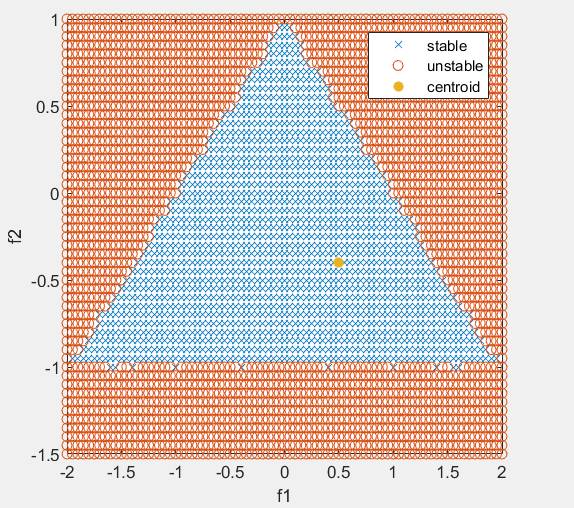
\includegraphics[width=0.4\textwidth]{figs/stability.PNG}\\
	\caption{AR Coefficient Stability Region}
	\label{stabf1f2}
\end{figure}

\subsection{Case 1: Static AR Processes}

In the static AR coefficient case, each row of the before mentioned data matrix contains an AR process generated with the same F matrix. Each row begins with a randomly generated sample with $\mu = 0$ and $\sigma^2 = 1$. Each row contains a different AR process but with the same AR coefficients. This format ensures that the TCN and KF both received a wide variety of AR processes that share the same coefficients but differ in starting value. In this case, both the training phase and testing phase data formats are the same. 

\subsection{Case 2: Varied AR Processes}

In the varied AR process case, each row of the data matrix contains a different AR process with differing coefficients, meaning that each row of the data matrix is associated with a unique F matrix.  The processes begin with the same conditions as in the first case:  $\mu = 0$ and $\sigma^2 = 1$. The variations in the F matrices are determined by a normal, Gaussian distribution about the chosen coefficient mean values. The reasoning for introducing this variation is that during the training phase, we wish to expose the model to as many AR processes as possible such that we obtain a network which is better capable of generalizing and extrapolating to other processes. 

For the mismatched data generation case where each row of the AR process matrix contains a different AR process generated by a normally distributed deviation from the chosen AR coefficient means, we obtain the heatmap of chosen coefficient values shown in Figure \ref{heatmap}. We discard any values which cause the eigenvalues of the F matrix to be larger than one, therefore the actual mean value of the coefficients deviates from what we use to generate the overall dataset. 

\begin{figure}[!h]
\centering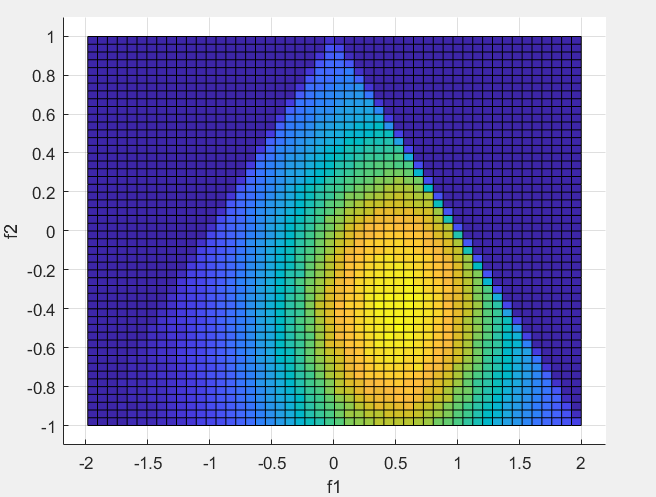
\includegraphics[width=0.3\textwidth]{figs/heatmap.PNG}\\
\caption{AR Coefficient Heatmap}
\label{heatmap}
\end{figure}

In testing, we wish to acquire better averages for resulting MSE values, therefore the AR process data matrices now contain AR processes in each row that share the same F matrix. With each iteration of testing, a new AR process data matrix is generated, with a different, normally distributed F matrix for the whole set of data.  

\subsection{Case 3: Gilbert-Elliott Model}

To construct the data for the burst noise Gilbert-Elliott channel of the form shown in Figure \ref{gbe}, we utilized a Markov chain for AR sequence generation. For every new sample generated, the Markov chain has a probability of transitioning from state to state $(P_{BG}, P_{GB})$ or staying where it is currently $(P_{BB}, P_{GG})$. The "bad" state here corresponds to a process generation scheme where the AR coefficients produce eigenvalues that are close to one, edging on the border between stability and instability while the "good" state is any other coefficient pair that resides close to the center of the triangle in Figure \ref{stabf1f2}. The complete AR sequence will have both transition regions with good and bad coefficients as well as consistent segments. We wish to challenge the linear estimators and neural network to recognize when the changes occur, as the optimum solution to this type of channel model would be two Kalman filters that can be switched between, depending on the current state. Upon each testing and training iteration, the generated sequence is formed into the following Toeplitz matrix structure:

$\vec{\textbf{X}} = \begin{bmatrix}
x[k-1]   & ...       & x[k-N-1]     & \\
x[k-2]   & ...       & x[k-N-2]     & \\
\vdots             &  \ddots   &              & \\
x[k-M-1] & ...       & x[k-M-N-1]  
\end{bmatrix}$

Then, this data is processed by each of the channel tracking systems. In the testing phase, we processed the AR sequence generated using the combination of good and bad coefficients, as well as obtained results for testing on either set separately. In choosing what constituted a "bad" set of coefficients, we simply chose an F matrix which contained an $f_1$ and $f_2$ pair which bordered the region of instability (resulting in a larger MMSE with the Ricatti), which in our case was the lower right-hand corner of the triangle in Figure \ref{stabf1f2}. 

\begin{figure}[!h]
\centering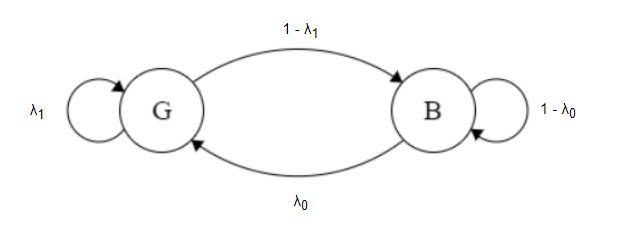
\includegraphics[width=0.45\textwidth]{figs/GBmodel.PNG}\\
\caption{Gilbert-Elliott Probabilistic Markov Chain}
\label{gbe}
\end{figure}

% ======================================
\section{Linear Estimators}
% ======================================
\label{sec:linest}

The most common approaches to accurately tracking the channel described in Section \ref{sec:channelmodel} use linear estimators such as the least squares solution or the Kalman filter. The LS solution is the most straightforward of the two and simply tries to find a line of best fit to the training data which is then used in further evaluations for test data. The KF on the other hand requires knowledge of the channel statistics such that a probabilistic estimation and prediction can be made of the current and next states. 

\subsection{Riccati Equation}

The Riccati equation allows us to have a lower bound for the best possible performance in channel estimation we could possibly have with a model mismatch, assuming access to an infinite dataset. In this specific case, this equation will always converge to a lower MSE than any other channel estimation method we are using (LS, KF, TCN). In the matched model case, the Riccati will simply verify that the KF is working properly, as they both converge to and provide the same solution. The Riccati in the discrete time domain is implemented with the following equation: 

$X=A^{\rm T}XF-(F^{\rm T}XH)(R+H^{\rm T}XH)^{-1}(H^{\rm T}XF) + Q $

\subsection{Least Squares}

Utilizing the least squares algorithm, we obtained filter coefficients which transform the measured state matrix (\textbf{Z}) into the best prediction or estimation ($\hat{x}$) that we can make given a sequence history of N and a filter order of M. The prediction/estimation and least squares coefficient solutions $(a_{ls}, b_{ls})$ are given by the following equations:
\begin{eqnarray*}
\hat{x_{est}}&=&\textbf{Z}a_{ls} \\ 
\hat{x_{pred}}&=&\textbf{Z}b_{ls} \\ 
a_{ls}&=&(\textbf{Z}^{\rm T}\textbf{Z})^{-1}\textbf{Z}^{\rm T}x_{est} \\
b_{ls}&=&(\textbf{Z}^{\rm T}\textbf{Z})^{-1}\textbf{Z}^{\rm T}x_{pred}
\end{eqnarray*}
\begin{align}
\begin{aligned}
x&= \left[ \begin{matrix}  x[k]   \dots    x[k-M] \end{matrix} \right]^\top\\
\hat{x_{pred}} &= \left[ \begin{matrix} \hat{x}[k-1]  \dots \hat{x}[k-M-1]\end{matrix} \right]^\top\\
\hat{x_{est}} &= \left[ \begin{matrix}   \hat{x}[k]  & \hat{x}[k-1]  &  \dots & \hat{x}[k-M]\end{matrix}\right]^\top\\ \nonumber
a_{ls}&=  \left[ \begin{matrix}    a_{0} &  a_{1} &  \dots  & a_{N} \end{matrix} \right]^\top\\
b_{ls}&= \left[ \begin{matrix}   b_{0}   & b_{1}  & \dots &  b_{N}\end{matrix}\right]^\top
\end{aligned}
\end{align}

$\vec{\textbf{Z}} = \begin{bmatrix}
   z[k-1]   & ...       & z[k-N-1]     & \\
   z[k-2]   & ...       & z[k-N-2]     & \\
   \vdots             &  \ddots   &              & \\
   z[k-M-1] & ...       & z[k-M-N-1]  
\end{bmatrix}$

The least squares filter coefficients are computed once using a training data sequence consisting of many segments of either one AR process or many, depending on the model being used. Both the mismatched and matched model cases are evaluated, with training occurring on large collections of AR processes and testing on individual, longer sequences. 

% Give the mathematics behind the least squares approach and how we designed it 

\subsection{Kalman Filter}

 We wish to estimate the current state as well as predict the future state of the AR process using the Kalman filter to compare performance of the TCN to a standard channel tracking system. To realize the KF in this situation, we used the following state update equations \cite{kay1993fundamentals}: \\
\begin{eqnarray*}
\hat{x}[n|n-1]&=&\textbf{F}\hat{x}[n-1|n-1] \\
\textbf{M}[n|n-1]&=&\textbf{FM}[n-1|n-1]\textbf{F}^{\rm T} + \textbf{Q} \\
\textbf{K}[n]&=&\frac{\textbf{M}[n|n-1]\textbf{H}}{\sigma_{w}^{2} + \textbf{H}^{\rm T}\textbf{M}[n|n-1]\textbf{H}} \\
\hat{x}[n|n]&=&\hat{x}[n|n-1] + \textbf{K}[n](z[n]-\textbf{H}^{\rm T}\hat{x}[n|n-1]) \\
\textbf{M}[n|n]&=&(\textbf{I}-\textbf{K}[n]\textbf{H}^{\rm T})\textbf{M}[n|n-1]
\end{eqnarray*}

\begin{table}[h!]
\centering
\begin{tabular}{|c|l|}
\hline
Notation           & Description \\ \hline              
\multirow{2}{*}{$\hat{x}[n|n-1]$} & \multirow{2}{*}{State prediction} \\
                   & \\ \hline
\multirow{2}{*}{$\hat{x}[n-1|n-1]$} & \multirow{2}{*}{Correction value} \\
                   & \\ \hline
\multirow{2}{*}{$\textbf{M}[n|n-1]$} & \multirow{2}{*}{Minimum prediction MSE} \\
                   & \\ \hline
\multirow{2}{*}{$\textbf{M}[n-1|n-1]$} & \multirow{2}{*}{Minimum estimation MSE} \\
                   & \\ \hline
\multirow{2}{*}{Q} & \multirow{2}{*}{Process noise} \\
                   & \\ \hline
\multirow{2}{*}{$\textbf{K}[n]$} & \multirow{2}{*}{Kalman gain} \\
                   & \\ \hline
\multirow{2}{*}{$\sigma_{w}^2$} & \multirow{2}{*}{Measurement noise covariance} \\
                   & \\ \hline
\end{tabular}
\end{table}

Generally, if the Kalman filter has perfect knowledge of the real AR coefficients, the MSE of this system will approach the Riccati equation MMSE. If the Kalman filter has an error in the assumed channel parameters however, it will result in a worse MSE than the Riccati.  In our case, we tested both circumstances; when the Kalman filter has perfect knowledge of the coefficients and also when there is a slight deviation. 

% ======================================
\section{Temporal Convolutional Network}
% ======================================
\label{sec:TCN}

The temporal convolutional network (TCN) is the neural network architecture we chose to design and test against the least squares and Kalman filter solutions. The TCN has proven to be more successful in sequence identification problems than recurrent neural networks (RNN) and long-short term memory neural networks (LSTM). The structure and general design of this neural network was provided by \cite{BaiTCN2018}, which we used and altered for channel estimation specific inputs and outputs. 

The TCN structure is essentially a one dimensional, fully connected network with causal convolutions. The main differences between a traditional convolutional neural network and the TCN are the diluted causal convolutions between network layers and the ability to specify a desired output sequence length. To accomplish this, the network contains hidden layers which are all of the same length and uses zero padding to keep the dilutions feasible and maintain the output size specification. Diluted convolutions increase the receptive field of each convolutional layer, providing the network the ability to account for sequence elements that are further back in the input history. 

\begin{figure}[!h]
	\centering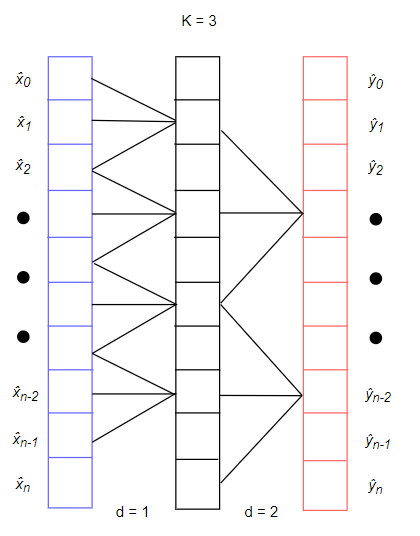
\includegraphics[width=0.3\textwidth]{figs/dilutedconv.png}\\
	\caption{Diluted Convolution Example}
	\label{dilutedconv}
\end{figure}

The TCN consists of multiple "residual blocks" which act as fundamental construction elements in this architecture. One instance of this network may consist of many residual blocks, all daisy-chaining in one long sequence. These residual blocks consist of two layers of diluted, causal convolutions and a non-linearity (ReLU) on the output of each layer. The residual blocks contain an identity mapping which aids in training for slight variations around the input sequence by explicitly weighting the output with a scaled version of the input before any convolutions took place. 

\begin{figure}[!h]
	\centering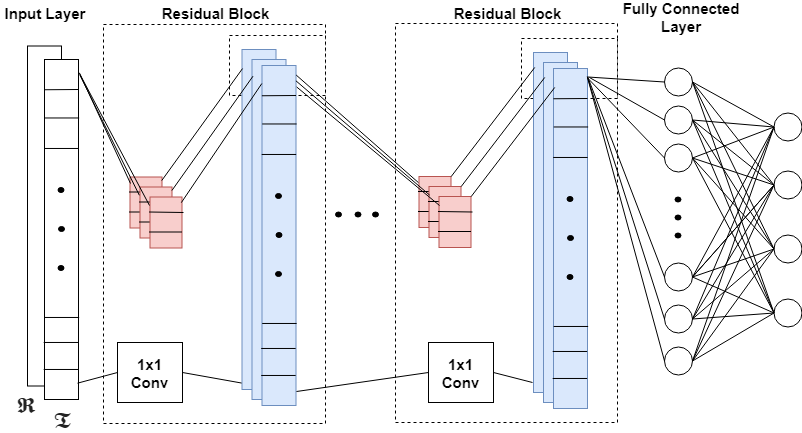
\includegraphics[width=0.5\textwidth]{figs/TCN.png}\\
	\caption{Temporal Convolutional Network Architecture}
	\label{TCNstruct}
\end{figure}

Due to the complex nature of the channel values, the imaginary and real components had to be split into separate numbers in order to effectively train the network. This splitting into real and imaginary components has already been done previously with favorable results \cite{tacspinar2010back}.  The loss function for this network is the mean-squared error (MSE), and for complex values this is calculated in the following way:
\begin{eqnarray*}
MSE&=&E(\lvert {x-\hat{x}}\rvert{^2}) \\
\end{eqnarray*}
Where $x$ and $\hat{x}$ are both complex valued states (actual and computed states, respectively). 


% ======================================
\section{Results}
% ======================================
\label{sec:results}

\subsection{Case 1: Static AR Processes}

\begin{table}[!h]
\begin{tabular}{|l|l|l|l|l|}
\hline
                            & MMSE                 & Least Squares        & Kalman         & TCN                   \\ \hline
\multirow{3}{*}{Estimation} & \multirow{3}{*}{ay}  & \multirow{3}{*}{doe} & \multirow{3}{*}{ay}   & \multirow{3}{*}{doe}  \\
                            &                      &                      &                       &                       \\
                            &                      &                      &                       &                       \\ \hline
\multirow{3}{*}{Prediction} & \multirow{3}{*}{aye} & \multirow{3}{*}{doe} & \multirow{3}{*}{ayez} & \multirow{3}{*}{doez} \\
                            &                      &                      &                       &                       \\
                            &                      &                      &                       &                       \\ \hline
\end{tabular}
\end{table}

\newpage

\subsection{Case 2: Varied AR Processes}

\begin{table}[!h]
\begin{tabular}{|l|l|l|l|l|}
\hline
                            & MMSE                 & Least Squares        & Kalman         & TCN                   \\ \hline
\multirow{3}{*}{Estimation} & \multirow{3}{*}{ay}  & \multirow{3}{*}{doe} & \multirow{3}{*}{ay}   & \multirow{3}{*}{doe}  \\
                            &                      &                      &                       &                       \\
                            &                      &                      &                       &                       \\ \hline
\multirow{3}{*}{Prediction} & \multirow{3}{*}{aye} & \multirow{3}{*}{doe} & \multirow{3}{*}{ayez} & \multirow{3}{*}{doez} \\
                            &                      &                      &                       &                       \\
                            &                      &                      &                       &                       \\ \hline
\end{tabular}
\end{table}


\subsection{Case 3: Gilbert-Elliott Model}

\begin{table}[!h]
\begin{tabular}{|l|l|l|l|l|}
\hline
                            & MMSE                 & Least Squares        & Kalman         & TCN                   \\ \hline
\multirow{3}{*}{Estimation} & \multirow{3}{*}{ay}  & \multirow{3}{*}{doe} & \multirow{3}{*}{ay}   & \multirow{3}{*}{doe}  \\
                            &                      &                      &                       &                       \\
                            &                      &                      &                       &                       \\ \hline
\multirow{3}{*}{Prediction} & \multirow{3}{*}{aye} & \multirow{3}{*}{doe} & \multirow{3}{*}{ayez} & \multirow{3}{*}{doez} \\
                            &                      &                      &                       &                       \\
                            &                      &                      &                       &                       \\ \hline
\end{tabular}
\end{table}

% This is the section in which the channel assumptions break down, meaning the Kalman Filter is estimating a channel which has a variance in the AR coefficients - the network is better here

% ======================================
\section{Conclusion}
% ======================================
\label{sec:conclusion}
This is the conclusion.

% Talk about the implications of the results - what they mean for us, where this research could go further, etc... 


All source code for this experiment is available at ---\\
\url{https://github.com/aspectlab/deepchannel}


% ------------------------------------------------------

%\vfill\pagebreak

%%%%%%%%%%%%%%%%%%%%%%%%%%%%%%%%%%%%%%%%%%%%%%%%%%%%%%%%%%%%%%%%%%%%%%%%%%%%%%%%%%%%%%%%%%%%%%%%%%%%%%
\acknowledgments
This work was supported by a Research Experience for Undergraduates
(REU) Supplement to National Science Foundation award CNS-1836695.


% -------------------------------------------------------------------------
\newpage
\bibliographystyle{IEEEtran}
\bibliography{IEEEabrv.bib,tcn_biblio.bib}

%%%%%%%%%%%%%%%%%%%%%%%%%%%%%%%%%%%%%%%%%%%%%%%%%%%%%%%%%%%%%%%%%%%%%%%%%%%%%%%%%%%%%%%%%%%%%%%%%%%%%%
\newpage
\thebiography
%% This biostyle allows you to insert your photo size 1in X 1.25in
\begin{biographywithpic}
{Arick Grootveld}{figs/grootveld.jpg}
is currently pursuing a B.S. in electrical engineering from WWU and expects to graduate in June 2020. His current research activities include... 
\lipsum[1-1]
\end{biographywithpic}

\begin{biographywithpic}
{Vlad Bugayev}{figs/bugayev.jpg}
is currently pursuing a B.S. in electrical engineering from WWU and expects to graduate in June 2020. His current research activities include ...
\lipsum[1-1]
\end{biographywithpic}

\begin{biographywithpic}
{Andrew G. Klein}{figs/klein.jpg}
received the B.S. degree from Cornell University, Ithaca,
NY, USA, the M.S. degree from the University of
California, Berkeley, CA, USA, and the Ph.D.
degree from Cornell University, all in electrical
engineering. Previously, he was an Assistant Professor with the Worcester Polytechnic Institute,
Worcester, MA, USA, from 2007 to 2014, and he
was a Post-Doctoral Researcher with Sup\'{e}lec/LSS,
Paris, France, from 2006 to 2007. He joined the
Department of Engineering and Design, Western
Washington University, Bellingham, WA, USA, in 2014, where he is currently
a Professor.
\end{biographywithpic}

\begin{biographywithpic}
{D. Richard Brown III}{figs/brown.jpg}
received the B.S. and M.S. degrees from the University of Connecticut in 1992 and 1996, respectively, and the Ph.D. degree from Cornell University
in 2000, all in electrical engineering. From 1992
to 1997, he was with General Electric Electrical
Distribution and Control. He was a Faculty Member
with the Worcester Polytechnic Institute, Worcester,
MA, USA, in 2000. He was a Visiting Associate
Professor with Princeton University from 2007 to
2008. From 2016 through 2018, he was with the Computing
and Communication Foundations Division, National Science Foundation, as
a Program Director.
\end{biographywithpic}

\begin{biographywithpic}
{Kirty Vedula}{figs/kpv.PNG}
Rutgers University, MS in Electrical and Computer Engineering, 2014 Amrita University, B Tech in Electronics and Communications Engineering, 2012. I joined the PhD in Electrical and Computer Engineering program in 2015. Prior to this, I completed my Master's degree at Rutgers University. I worked at Mathworks (Framingham, MA) and Visible Energy(Palo Alto, CA) earlier. My research interests are in signal processing, wireless communication systems, wireless power transfer and hardware security.
\end{biographywithpic}


\end{document}
